\documentclass[a4paper,11pt,final]{article}


\usepackage{listings}

% Include all necessary packages

\usepackage{listings}								% For code segments
\usepackage{color}									% For text, links and code highlighting
\usepackage[pdftex]{hyperref}						% For external and internal links
\usepackage{graphicx}								% For including figures
\usepackage[utf8]{inputenc}							% The package translates various standard and other input encodings into a ‘LaTeX internal language’
\usepackage[T1]{fontenc}							% The package allows the user to select font encodings, and for each encoding provides an interface to ‘font-encoding-specific’ commands for each font.
\usepackage{sectsty}								% A LaTeX2e package to help change the style of any or all of LaTeX's sectional headers in the article, book, or report classes. 
\usepackage[french]{babel}							% The package manages culturally-determined typographical (and other) rules, and hyphenation patterns for a wide range of languages.
\usepackage{geometry}								% The package provides an easy and flexible user interface to customize page layout   
\usepackage{textcomp}								% Supports the Text Companion fonts which provide many text symbols (such as baht, bullet, copyright, musicalnote, onequarter, section, and yen) in the TS1 encoding. 
\usepackage[toc, acronym,style=altlist]{glossaries}	% For build glossary and include an internal link into the table of content. 
\usepackage{index}									% For index.
\usepackage{caption}								% For caption customization

\usepackage{setspace}
\usepackage{hyperref}
%\usepackage[french]{varioref}
\usepackage{setspace}
\usepackage[french]{babel}
\usepackage{fancyhdr}
\usepackage{lastpage}
\usepackage{fancybox}
\usepackage{float}
\usepackage{verbatimbox}


%\usepackage[final]{pdfpages}						% This package simplifies the insertion of external multi-page PDF or PS doc-uments. It supports pdfTeX, VTeX, and XeTeX.
\usepackage{float}									% Improves the interface for defining floating objects such as figures and tables.

\usepackage{amsmath}								% It adapts for use in LaTeX most of the mathematical features found in AMS-TeX
\usepackage{amssymb}								% This file defines all the symbols found in the AMS symbol fonts msam and msbm.
%\usepackage{mathrsfs}

\usepackage{array,longtable}						% Longtable allows you to write tables that continue to the next page
%\usepackage{rotating}								% A package built on the standard LaTeX graphics package to perform all the different sorts of rotation.

\usepackage{amstext}
\usepackage{latexsym}
\usepackage{epsf} 
\usepackage{amsfonts}
\usepackage{sansmath}

\usepackage{stmaryrd}


% Personal command
\newcommand{\MG}{\mathcal{G}}
\newcommand{\ML}{\mathcal{L}}
\newcommand{\MN}{\mathcal{N}}
\newcommand{\MU}{\mathcal{U}}
\newcommand{\MQ}{\mathcal{Q}}
\newcommand{\e}{\mathrm e}
\newcommand{\ind}{\mathbf{1}}
\newcommand{\EMMTETA}{\tilde \theta_{n}}
\newcommand{\XNB}{\bar{X}_{n}}
\newcommand{\dx}{\,dx}
\newcommand{\dt}{\,dt}
\newcommand{\R}{\mathbb{R}}
\newcommand{\N}{\mathbb{N}}
\newcommand{\abs}[1]{\left\lvert#1\right\rvert}
\newcommand{\norm}[1]{\left\lVert#1\right\rVert}


% Personal color definitions

\definecolor{P_GREEN}		{rgb}	{0.0,0.45,0.0}	% Light green 
\definecolor{P_ORANGE}		{rgb}	{1.00,0.65,0.20}	% Light orange
\definecolor{P_GREY}		{rgb}	{0.45,0.45,0.45}	% Medium grey (Eolas grey)
\definecolor{P_BROWN}		{rgb}	{0.40,0.0,0.0}
\definecolor{P_BLUE_DARK}		{rgb}	{0.00, 0.00, 0.205}	% Medium blue (Eolas blue)
\definecolor{P_BLUE}		{rgb}	{0.0, 0.0, 0.40}
%\definecolor{P_BLUE_LIGHT}		{rgb}	{0.33, 0.5, 0.93}
\definecolor{P_BLUE_LIGHT}		{rgb}	{0.0, 0.0, 0.63}
\definecolor{P_RED}			{rgb}	{0.63,0.13,0.13} 	% Dark red (scarlet red)

% Style & color settings

% Style & color for input name in the glossary (blod & light green)
\renewcommand{\glsnamefont}[1]{\color{P_GREEN}{\textbf{#1}}}

% Color of captions (figures, listing, tables) (medium grey)
\captionsetup {
  font = {
    color = P_GREY
  }
}


% Color for each structure part
%%\titlefont     {\color{P_GREY}}
\partfont	 		{\color{P_GREY}}	% Part are set in medium grey
\chapterfont		{\color{P_GREY}}	% Chapter are set in medium grey
\sectionfont		{\color{P_GREEN}}	% Section are set in light green
\subsectionfont		{\color{P_BLUE}}	% Subsection are set in light orange
\subsubsectionfont	{\color{P_BLUE_LIGHT}}	% Subsubsection are set in medium grey



% Table of Content customization

%%
% 	Each sectiontype (chapter, section, ...) has a number associated with it. Two other counters determine when section numbers are printed (secnumdepth) and what sections appear in the table of contents (tocdepth). 
%	Part			=	-1
%	Chapter			=	0
%	Section 		= 	1
%	Subsection		=	2
%	Subsubsection	=	3
%	Paragraph		=	4
%	Subparagraph	=	5
%	
%\setcounter{secnumdepth}{0}	% Chapter are printed
%\setcounter{tocdepth}{4}   	% List parts, chapters, sections, subsections, and subsubsections in the table of contents
%%

% Personnal commands definitions

% Draw an horizontal rule, width of 0.1mm
\newcommand{\HRule} {
  \rule{\linewidth}{0.1mm}
}

% Glossary, index creation

\makeglossaries % Allow glossary creation
\makeindex		% Allow index creation

% Personal link and PDF definitions

\hypersetup{
  pdffitwindow	=	false,     				% Page fit to the window when opened
  %
  pdftitle		=	{Compte rendu},    	% PDF Title (show in reader bar)
  pdfauthor		=	{noname},	% PDF author (show in PDF properties)
  pdfsubject		=	{Test},  				% PDF subject (show in PDF properties)
  pdfkeywords		=	{sample} {example},		% List of keywords (show in the PDF properties)
  pdfcreator		=	{noname},   	% Creator of the PDF (show in the PDF properties)
  pdfproducer		=	{noname},	% Producer of the PDF (show in the PDF properties)
  %
  colorlinks		=	true,       			% False : boxed links; true: colored links
  urlcolor		=	P_BLUE,          		% Color of external links
  linkcolor		=	black,          		% Color of internal links
  citecolor		=	black,        			% Color of links to bibliography
  filecolor		=	black,      			% Color of file links
  %
  pdfnewwindow	=	true      				% Links are displayed / or not in new window
  %
  %bookmarks		=	true,         			% Show / or not bookmarks bar
  %unicode		=	false,          		% Non-Latin characters in Acrobat’s bookmarks
  %pdftoolbar		=	true,        			% Show / or not Acrobat’s toolbar
  %pdfmenubar		=	true,        			% Show / or not Acrobat’s menu
  %pdfstartview	=	{FitH},    				% Fits the width of the page to the window
  %
}

% Personal listing / code definitions

% General settings for listings
\lstset{ %
  %language			=, 														% Set the language of the code
  %
  title				=	\lstname, 											% Show the filename of files included with \lstinputlisting
  caption				=	\lstname,
  %
  frame				=	single, 											% Set / or not the frame style around the code
  backgroundcolor		=	\color{white}, 										% Background color
  %
  basicstyle			=	\footnotesize, 										% Set the size of the font that are used for the code
  %
  breaklines			=	true,												% Allow automatic breakline instead of overflow the listing size limits
  breakindent			=	10pt,												% Indent between code and break character
  breakatwhitespace	=	true,												% Break only on space (not during a word)
  breakautoindent		=	true,                         						% Auto indent after breaking
  prebreak			=	\raisebox{0ex}[0ex][0ex]{\ensuremath{\backslash}},	% Set the character before breaking (ex: int main \)
  %
  %numbers			=	left, 												% Where to put the line-numbers
  %numberstyle		=	\footnotesize, 										% Set the site of the font that are used for lines numbering
  %stepnumber			=	1, 													% Step between two line-number
  %numbersep			=	5pt,												% Indentation between line-numbers and code
  %numberblanklines	=	true,												% Numbering or not blank lines
  %
  showspaces			=	false, 												% Replace / or not spaces by particular underscores
  %showstringspaces	=	false, 												% Underline spaces within strings
  %showtabs			=	false, 												% Replace / or not tabs by particular underscores
  tabsize				=	4, 													% Sets default tabsize to 2 spaces
  %
  captionpos			=	b 													% Set the caption position (b = bottom, t = top, ...)
  %
}

% Add the CLI as a language for listing
\lstdefinelanguage{cli} {
  morekeywords={install},		
  otherkeywords={apt-get},
  morecomment=[l]\#,			% Each begining with the '#' char is set as an comment
  %
  keywordstyle=\color{P_GREEN},	
  commentstyle=\color{P_RED}
}

\lstset{
  morekeywords={abort,abs,accept,access,all,and,array,at,begin,body,
    case,constant,declare,delay,delta,digits,do,else,elsif,end,entry,
    exception,exit,for,function,generic,goto,if,in,is,limited,loop,
    mod,new,not,null,of,or,others,out,package,pragma,private,
    procédure,raise,range,record,rem,renames,return,reverse,select,
    separate,subtype,task,terminate,then,type,use,when,while,with,
    xor,abstract,aliased,protected,requeue,tagged,until},
  sensitive=f,
  morecomment=[l]--,
  morestring=[d]",
  showstringspaces=false,
  basicstyle=\small\ttfamily,
  keywordstyle=\bf\small,
  commentstyle=\itshape,
  stringstyle=\sf,
  extendedchars=true,
  columns=[c]fixed
}


\lstset{
  literate=%
  {À}{{\`A}}1 {Â}{{\^A}}1 {Ç}{{\c{C}}}1%
  {à}{{\`a}}1 {â}{{\^a}}1 {ç}{{\c{c}}}1%
  {É}{{\'E}}1 {È}{{\`E}}1 {Ê}{{\^E}}1 {Ë}{{\"E}}1% 
  {é}{{\'e}}1 {è}{{\`e}}1 {ê}{{\^e}}1 {ë}{{\"e}}1%
  {Ï}{{\"I}}1 {Î}{{\^I}}1 {Ô}{{\^O}}1%
  {ï}{{\"i}}1 {î}{{\^i}}1 {ô}{{\^o}}1%
  {Ù}{{\`U}}1 {Û}{{\^U}}1 {Ü}{{\"U}}1%
  {ù}{{\`u}}1 {û}{{\^u}}1 {ü}{{\"u}}1%
}


\setlength{\parindent}{0pt}
\setlength{\parskip}{1ex}
\setlength{\textwidth}{17cm} 
\setlength{\textheight}{23cm} 
\setlength{\oddsidemargin}{-.1cm}  %%
\setlength{\evensidemargin}{-.1in} %%
\setlength{\topmargin}{-.6in}

\newcommand{\reporttitle}{Inférence statistique des copules}     % Titre
\newcommand{\reportauthor}{Yacov \textsc{Hamou},\\ Jean \textsc{Lejay},\\ Guillaume \textsc{Palvadeau},\\Christophe \textsc{Pelet}} % Auteur
\newcommand{\reportsubject}{Projet - M2 SAF} % Sujet
\setlength{\parskip}{1ex} % Espace entre les paragraphes

\hypersetup{
    pdftitle={\reporttitle},%
    pdfauthor={\reportauthor},%
    pdfsubject={\reportsubject},%
    pdfkeywords={rapport} {vos} {mots} {clés}
}


%%%%%%%%%%%%%%% Début du document %%%%%%%%%%%%%%%%%%%%%%%%%%%%%%%%%%%%%%%

\begin{document}

 \begin{titlepage}

\begin{center}

%% \begin{minipage}[t]{0.48\textwidth}
%%   \begin{flushright}
%%     \includegraphics [width=30mm]{images/logo-societe.jpg} \\[0.5cm]
%%     \textsc{\LARGE Entreprise}
%%   \end{flushright}
%% \end{minipage} \\[1.5cm]

%% ~\vspace*{6cm}

~\vspace*{5mm}

\begin{minipage}[t]{0.48\textwidth}
  \begin{flushleft}
    \centering \includegraphics [width=8cm]{images/presentation3.png} \\[0.5cm]
    \begin{spacing}{1.5}
      %% \textsc{\LARGE École nationale supérieure d'informatique et de
      %%   mathématiques appliquées de Grenoble}
    \end{spacing}
  \end{flushleft}
\end{minipage}

~\vspace*{12mm}

\textsc{\Large \reportsubject}\\[0.5cm]
\HRule \\[0.4cm]
{\huge \bfseries \reporttitle}\\[0.4cm]
\HRule \\[1.5cm]

\begin{minipage}[t]{0.3\textwidth}
  \begin{flushleft} \large
    \emph{Auteurs :}\\
    \reportauthor
  \end{flushleft}
\end{minipage}
\begin{minipage}[t]{0.6\textwidth}
  \begin{flushright} \large
    \emph{Responsable :} \\
    TODO \\%M.~Christian \textsc{Robert} \\
    %% M.~Pierre \textsc{Bidon}
  \end{flushright}
\end{minipage}

\vfill

~\vspace*{14mm}

\begin{minipage}[t]{0.48\textwidth}
  \begin{flushleft}
    \centering \includegraphics [width=15mm]{images/logo-isfa.jpg} \\[0.5cm]
    \begin{spacing}{1.5}
      %% \textsc{\LARGE École nationale supérieure d'informatique et de
      %%   mathématiques appliquées de Grenoble}
    \end{spacing}
  \end{flushleft}
\end{minipage}

%~\vspace*{1mm}

{\large 28 Avril 2015}

\end{center}

\end{titlepage}

  \cleardoublepage % Dans le cas du recto verso, ajoute une page blanche si besoin
  \tableofcontents % Table des matières
  \sloppy          % Justification moins stricte : des mots ne dépasseront pas des paragraphes

\cleardoublepage  
\listoffigures  % table des figures
\cleardoublepage  
\listoftables   % table des tableaux



  %\cleardoublepage
  \section*{Introduction} % Pas de numérotation
\addcontentsline{toc}{section}{Introduction} % Ajout dans la table des matières

La théorie des copules a connu ces trois dernières décennies un essor considérable.
Ce développement a notamment vu ses applications de plus en plus nombreuses dans le domaine de la finance.
La gestion des risques, l'évaluation des rendements d'actifs, la théorie des valeurs extrêmes, requièrent des modélisations de
la dépendance et la théorie des copules permet à la finance d'accomoder la non-normalité des variables.

Avec une grande souplesse dans la mise en oeuvre de l'analyse multivariée, les copules autorisent une  sélection plus étendue des distributions conjointes des séries de données.
Les fonctions copules permettent une représentation moins naïve de la dépendance statistique fondée sur la mesure traditionnelle de corrélation qui présente des limites dans l'étude de l'interdépendance entre deux variables (cf. Embrechts et al. (1999)). 
En outre, elles autorisent des distributions de probabilités jointes moins restrictives, prenant  mieux en compte certaines caractéristiques comme l'asymétrie ou la dépendance de queue.
En somme, elles permettent de construire des distributions multidimensionnelles assez générales indépendamment des lois des marginales.

Dans ce projet, nous utiliserons cet outil puissant afin de modéliser au mieux la dépendance existant entre deux séries de données relatives 
à la vitesse maximale du vent relevées dans deux stations différentes mais proches géographiquement.

Dans une première partie, nous chercherons à décrire les données en présence et la dépendance sous-jacente au moyen de graphiques et de mesures de dépendance.
Puis, dans une seconde partie nous présenterons la copule empirique calculée sur nos données et qui nous servira de référentiel lors des tests à venir. Après un rappel théorique en début de chaque section, les parties qui suivront mettront en application différentes méthodes d'estimation sur des copules archimédiennes et des copules elliptiques :

\begin{itemize}
\item la méthode semi-paramétrique CML (Canonical Maximum Likelihood),
\item la méthode des moments,
\item les méthodes paramétriques, telles que la méthode du maximum de vraisemblance et la méthode IFM (Inference Function for Margins).
\end{itemize} 

Ensuite, nous réaliserons différents tests graphiques d'adéquation aux copules étudiées et des tests statistiques afin de retenir ou non l'adéquation des modèles de copule à nos données. 

L'ensemble des algorithmes et applications numériques ont été réalisés dans le langage de programmation $R$, dont le code est fourni avec le présent mémoire.
  
  \cleardoublepage
  
\section{Données}
%%%%%%%%%%%%%%%%%%%%%%%%%%%%%%%%%%%%%%%%%%%%%%%%%%%%%%%%%%%%%%%%%%%%%%%
\subsection{Présentation}

Nous disposons de deux séries de données contenues dans le package \lstinline!gumbel! correspondant à la vitesse maximale du vent par jour, sur la période août 2005 - avril 2007,
relevée à deux stations différentes en région Rhône-Alpes : l'une à Saint Martin en haut (département du Rhône) et et une autre à Echirolles (département de l'Isère).

~\\~
Notons :
\begin{itemize}
\item $(X_t)_t$ la série relative à la force maximale du vent (en m/s) par jour relevée par la station à Saint Martin en Haut 
\item $(Y_t)_t$ la série relative à la force maximale du vent (en m/s) par jour relevée par la station à Echirolles.
\end{itemize}

~\\~
Puisque les jeux de données appelés dans $R$ \lstinline!windEchirolles! et \lstinline!windStMartin! possèdent 
un nombre d’enregistrements différents en 2007, nous sélectionnons le plus petit sous-ensemble. Les données manquantes sont aussi retirées de la série.

Nous avons ainsi deux vecteurs de données contenant chacun $T=633$ données (correspondant à 633 jours).


\subsection{Formalisation}

Nous allons donc nous intéresser à la relation existant entre ces deux variables aléatoires réelles au moyen de modélisations par copules.
En effet,  les fonctions copules permettent de déterminer la nature de dépendance des séries qu’elle soit linéaire ou pas, monotone ou pas.

D'une manière explicite, les copules sont des fonctions de répartition particulières,
qui lient les fonctions de répartition multivariéees de lois de probabilitée dans $\mathbb{R}^d$, où $d \geq 2$ (ici $d$ sera égal à 2 car nous aurons un modèle bivarié) aux fonctions de répartition marginales de leurs coordonnées. 
La caractéristique des copules permet de séparer les distributions marginales de la structure de dépendance.

Plus précisément, $X$ et $Y$  sont définies sur un espace de probabilité $(\Omega,\mathcal{A},\mathbb{P})$, de fonction de répartition conjointe $H$ et de marginales $F$ et $G$.

D'après Sklar (1959), il existe une fonction de répartition bivariée $C$ dont les marges sont uniformes sur $[0,1]$, telle que :
$$
H(x,y) = C(F(x),G(y))
$$

De plus, si $F$ et $G$ sont continues, la copule $C$ est alors unique et on a :

$$
\forall (u,v) \in [0,1]^2 ~~ C(u,v) = H(F^{-1}(u),G^{-1}(v))
$$

En fait, il s'agit de la loi du couple $(U,V) = (F(X),G(Y))$.

Nous allons donc chercher la copule qui s’adapte le mieux à nos données.




\subsection{Observation graphique}



\subsubsection{Scatter plot}




\subsubsection{Rank-rank plot}

\subsection{Mesurer la dépendance}

\subsubsection{Dépendance ou corrélation ?}

Il est important de rappeler que les notions de dépendance et de corrélation sont différentes.
En effet, si $X$ et $Y$ sont indépendantes, cela implique que $X$ et $Y$ sont non corrélées. Mais attention, la réciproque est fausse, sauf dans
le cas où les variables sont gaussiennes car la dépendance est alors entièrement caractérisées par le coefficient de corrélation.

Un contre-exemple permettant d'illustrer cette remarque est le suivant :

Soit $X \sim \mathcal{N}(0,1)$ et $Y = X^2$, alors $\operatorname{Cov}(X,Y) = E[X^3] = 0$.

Le coefficient de corrélation doit donc être utilisée avec précaution car il n’est pertinent qu’en présence de distributions elliptiques (distribution multivariée
Normale ou de Student) ou de dépendance linéaire.


\subsubsection{Corrélation de Pearson}

Le coefficient de corrélation linéaire de Pearson est défini, pour nos deux variables aléatoires $X$ et $Y$ de variances finies, par :

$$
\rho(X,Y) = \frac{\operatorname{Cov}(X,Y)}{\sqrt{ \operatorname{Var}(X) \operatorname{Var}(Y)}}
$$

où $\operatorname{Cov}(X,Y) = E[XY] - E[X] E[Y]$ est la covariance entre $X$ et $Y$ et $\operatorname{Var}(X)$, $\operatorname{Var}(Y)$ correspondent aux variances respectives
de $X$ et $Y$.

On a alors :

\begin{itemize}
\item $X$ et $Y$ sont corrélées linéairement $\Longleftrightarrow \rho(X,Y) \neq 0$
\item $X$ et $Y$ sont non corrélées linéairement $\Longleftrightarrow \rho(X,Y) = 0$
\end{itemize}

Le coefficient de corrélation de Pearson est la mesure la plus connue. Mais il constitute une mesure très imparfaite de la dépendance. Il ne
peut se mettre sous une forme ne faisant intervenir que la copule, les marginales restent présentent dans l’expression : ce coefficient n’est donc
pas une mesure de dépendance.

De plus, il n’intègre que la composante linéaire de la dépendance, au sens où $r(X,Y) \pm 1$ si et seulement si $Y= a \times x + b$.

Enfin, on peut montrer (en utilisant l'inégalité de Tchen) que, pour les marginales fixées, toutes les valeurs
comprises entre -1 et +1 ne sont pas atteignables.

Ainsi, on retiendra que ce coefficient mesure mal une association non-linéaire, qu'il est trop sensible aux valeurs extrêmes et qu'il ne mesure pas vraiment la distance à l'indépendance.

Pour remédier à cela, nous avons recours à d’autres indicateurs de dépendance se basant sur les rangs et les concordances observés de notre échantillon de données. 
Ainsi, nous utilisons des coefficients de corrélation non linéaires, comme le rhô de Spearman ou le tau de Kendall.

\subsubsection{Rhô de Spearman}

Le rhô de Spearman $\rho_S$ se définit comme la corrélation entre les rangs d'observations.

Soient $X=(X_1,...,X_n)$ et $Y=(Y_1,...,Y_n)$ deux vecteurs aléatoires réels et $R = (R_1,...,R_n)$ et $S = (S_1,...,S_n)$ les vecteurs aléatoires des rangs respectivement
de $X$ et $Y$, alors :

$$
\rho_s = \rho(R,S) = \frac{\operatorname{Cov}(R,S)}{\sqrt{ \operatorname{Var}(R) \operatorname{Var}(S)}} = \frac{ \sum_{i=1}^n (R_i - \bar{R}) \times (S_i - \bar{S})  }{ \sqrt{   \sum_{i=1}^n (R_i - \bar{R})^2 \times  \sum_{i=1}^n (S_i - \bar{S})^2    }    }
$$

De plus, $rho_s$ vérifie les propriétés suivantes :

\begin{enumerate}

\item $\rho_s(X,Y) = \rho_s(Y,X), ~~\forall (X,Y)$
\item $|\rho_s(X,Y)| \leq 1, ~~\forall (X,Y)$
\item 
\begin{itemize}
\item $X$ et $Y$ comonotones $\Longleftrightarrow \rho_s(X,Y)=1$
\item $X$ et $Y$ antimonotones $\Longleftrightarrow \rho_s(X,Y)=-1$
\end{itemize}
\item Si $g$ est une fonction strictement croissante alors $\rho_s(g(X),g(Y))=\rho_s(X,Y)$.

\end{enumerate}

En revanche, et communément à la corrélation de Pearson, il n’y a pas d’équivalence entre non-corrélation et indépendance :
$$
X \text{~et~} Y \text{~indépendantes~} \Longrightarrow \rho_s(X,Y) = 0
$$
	
Le $\rho$ de Spearman élimine par construction l’effet de dépendance aux lois marginales.


\subsubsection{Tau de Kendall}

Soit $(X,Y)$ un vecteur aléatoire et $(X',Y')$ une copie de ce même vecteur. Le tau de Kendall $\tau$ est défini
comme la différence  entre les probabilités de concordance et de discordance entre $(X,Y)$ et $(X',Y')$ :

$$
\tau(X,Y) = P\left( (X-X')(Y-Y') >0 \right) - P\left( (X-X')(Y-Y') <0 \right)
$$

Notons que $\tau$ est une fonction des rangs des observations car, en notant $R$, $R'$, $S$, $S'$ les rangs de $X$, $X'$, $S$ et $S'$ respectivement, on a 
$$
(X-X')(Y-Y') >0 \Longleftrightarrow (R-R')(S-S') >0 
$$

En outre, $\tau$ vérifie les propriétés suivantes :

\begin{enumerate}

\item $\tau(X,Y) = \tau(Y,X), ~~\forall (X,Y)$
\item $|\tau(X,Y)| \leq 1, ~~\forall (X,Y)$
\item 
\begin{itemize}
\item $X$ et $Y$ comonotones $\Longleftrightarrow \tau(X,Y)=1$
\item $X$ et $Y$ antimonotones $\Longleftrightarrow \tau(X,Y)=-1$
\end{itemize}
\item Si $g$ est une fonction strictement croissante alors $\tau(g(X),g(Y))=\tau(X,Y)$.
\end{enumerate}

Enfin, comme les deux mesures précédentes, on a :

$$
X \text{~et~} Y \text{~indépendantes~} \Longrightarrow \tau(X,Y) = 0
$$



\section{Méthode non paramétrique d'estimation : la copule empirique}
%%%%%%%%%%%%%%%%%%%%%%%%%%%%%%%%%%%%%%%%%%%%%%%%%%%%%%%%%%%%%%%%%%%%%%%
\subsection{Choix d'une copule théorique}




\section{Méthode paramétriques d'estimation}
%%%%%%%%%%%%%%%%%%%%%%%%%%%%%%%%%%%%%%%%%%%%%%%%%%%%%%%%%%%%%%%%%%%%%%%

Dans cette section, nous allons présenter et utiliser deux méthodes paramétriques d'estimation
des copules :

\begin{itemize}
\item la méthode du maximum de vraisemblance
\item la méthode IFM (Inference Function for Margins).
\end{itemize}

\subsection{Méthode du maximum de vraisemblance}

\subsection{Méthode IFM (Inference Function for Margins)}


\section{Méthode semi-paramétrique d'estimation (CML)}
%%%%%%%%%%%%%%%%%%%%%%%%%%%%%%%%%%%%%%%%%%%%%%%%%%%%%%%%%%%%%%%%%%%%%%%

Dans cette section, nous allons utiliser la méthode CML (Canonical Maximum Likelihood, méthode semi-paramétrique) afin d'estimer le paramètre des différentes copules retenues pour modéliser la dépendance entre les données sur Saint-Martin et celles sur Echirolles.
En effet, à l'aide de cette méthode, on peut obtenir une estimation du paramètre de la copule sans se soucier des marginales. Pour cela, il suffit d'utiliser la fonction \textit{fitcopula} de R en passant comme arguments les rangs sur nos deux groupes de données translatés sur $[0;1]$ et un point de départ de l'algorithme. Ce point de départ sera l'estimation du paramètre de la copule obtenue par la méthode des moments. Avec l'estimation du paramètre obtenue en sortie de notre algorithme, on peut alors créer notre copule estimée.

\subsection{Copule de Clayton}

Dans le cas de la copule de Clayton, on obtient, en sortie de l'algorithme, $\widehat{\theta}_{CML}=0,70851$ comme estimation du paramètre de la copule. L'écart type pour cet estimateur vaut $sd = 0,069$. La valeur obtenue pour l'estimation du paramètre est donc significative. Le maximum de vraisemblance est de $72,25$. 
On peut ainsi tracer les Khi-plot et K-plot de cette copule de Clayton estimée et comparer les graphes avec ceux obtenus pour la copule empirique.

\noindent%
\begin{figure}[H]
    \begin{center}
      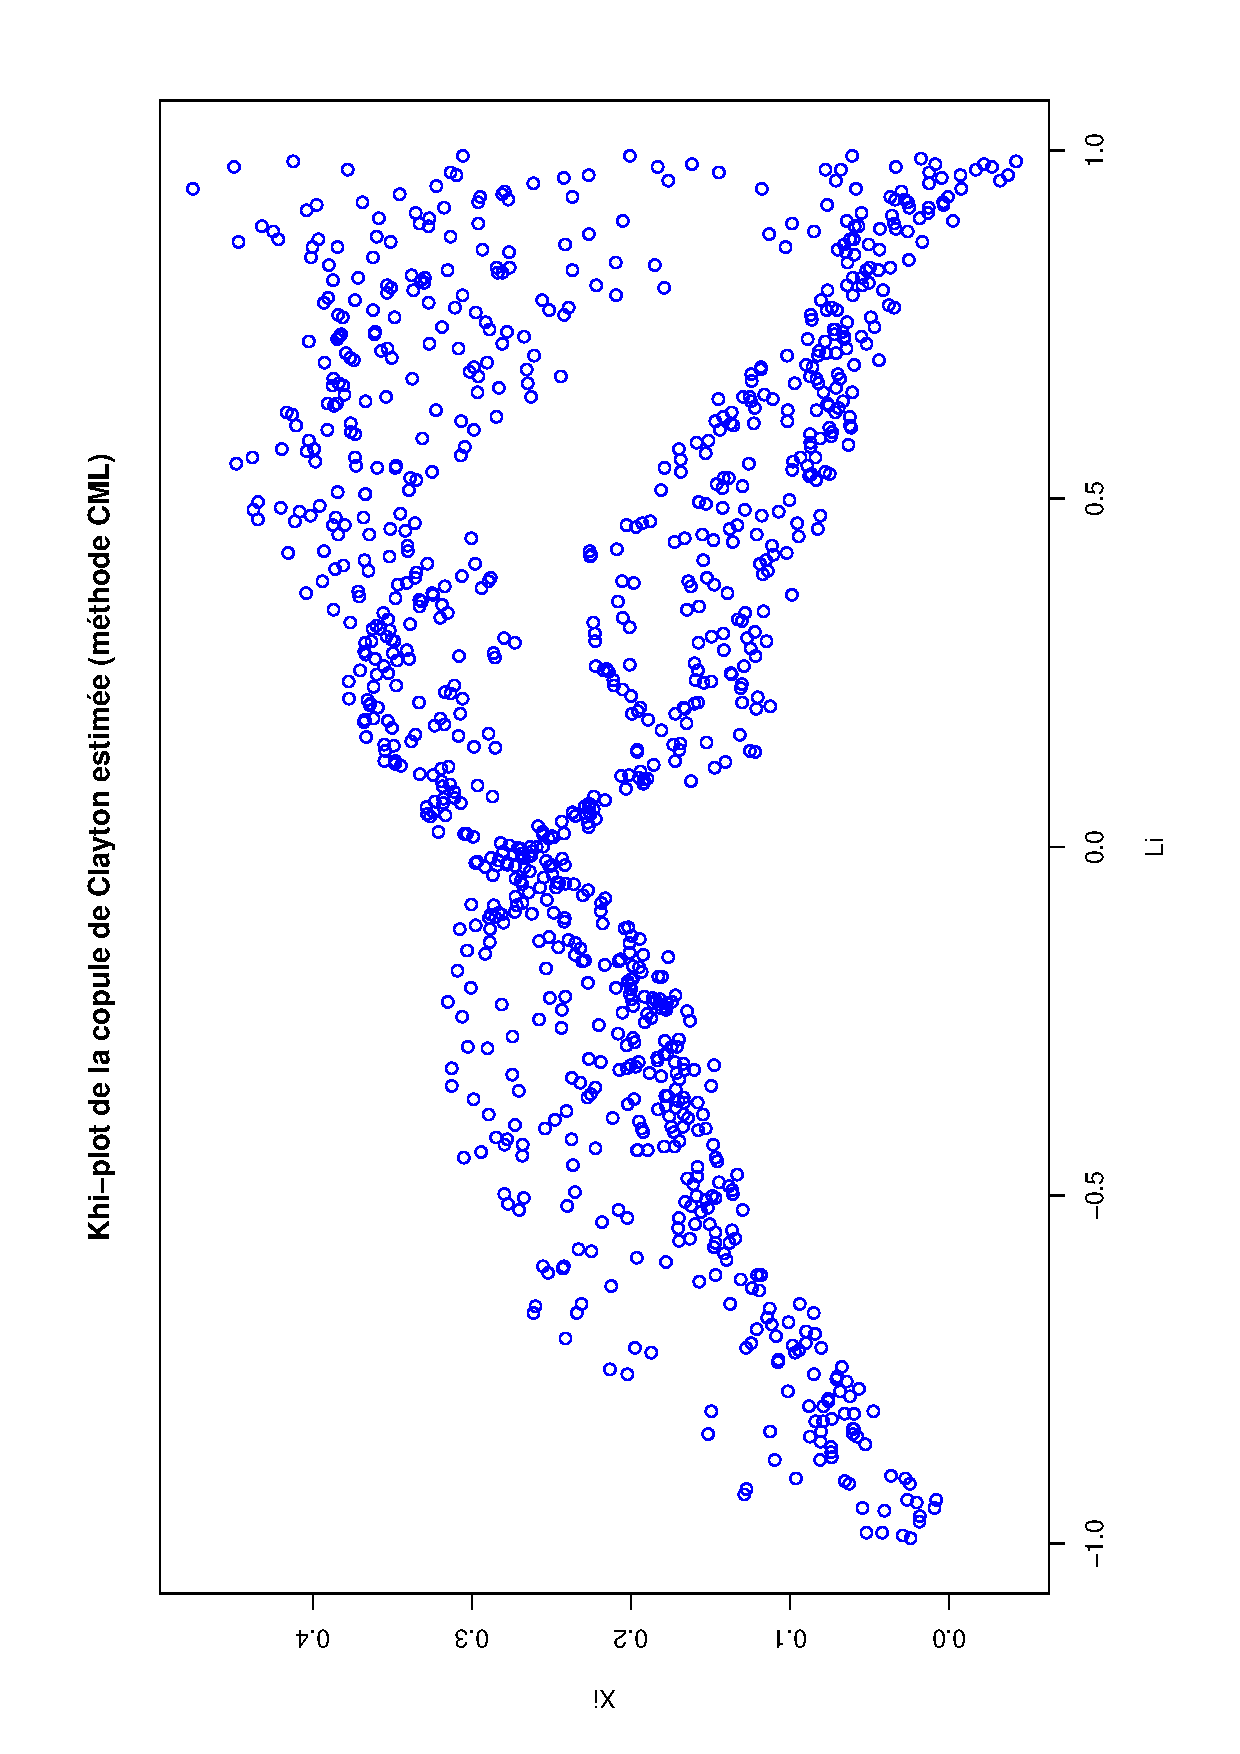
\includegraphics[width=17 cm, angle=0]{./pictures/claytoncmlkhiplot.png}
      \centering\caption{\label{2}Khi-plot de la copule de Clayton estimée (méthode CML)}
    \end{center}
\end{figure}

En comparant ce graphe du Khi-plot avec celui obtenu pour la copule empirique, on peut apercevoir une ressemblance, notamment dûe au fait que les points se répartissent du même côté de l'axe des ordonées (du côté positif) exprimant ainsi une dépendance positive. Cependant, du côté positif de l'axe des abscisses, le nuage de point semble se séparer en deux. Ceci n'est pas observée sur le Khi-plot de la copule empirique. 

\noindent%
\begin{figure}[H]
    \begin{center}
      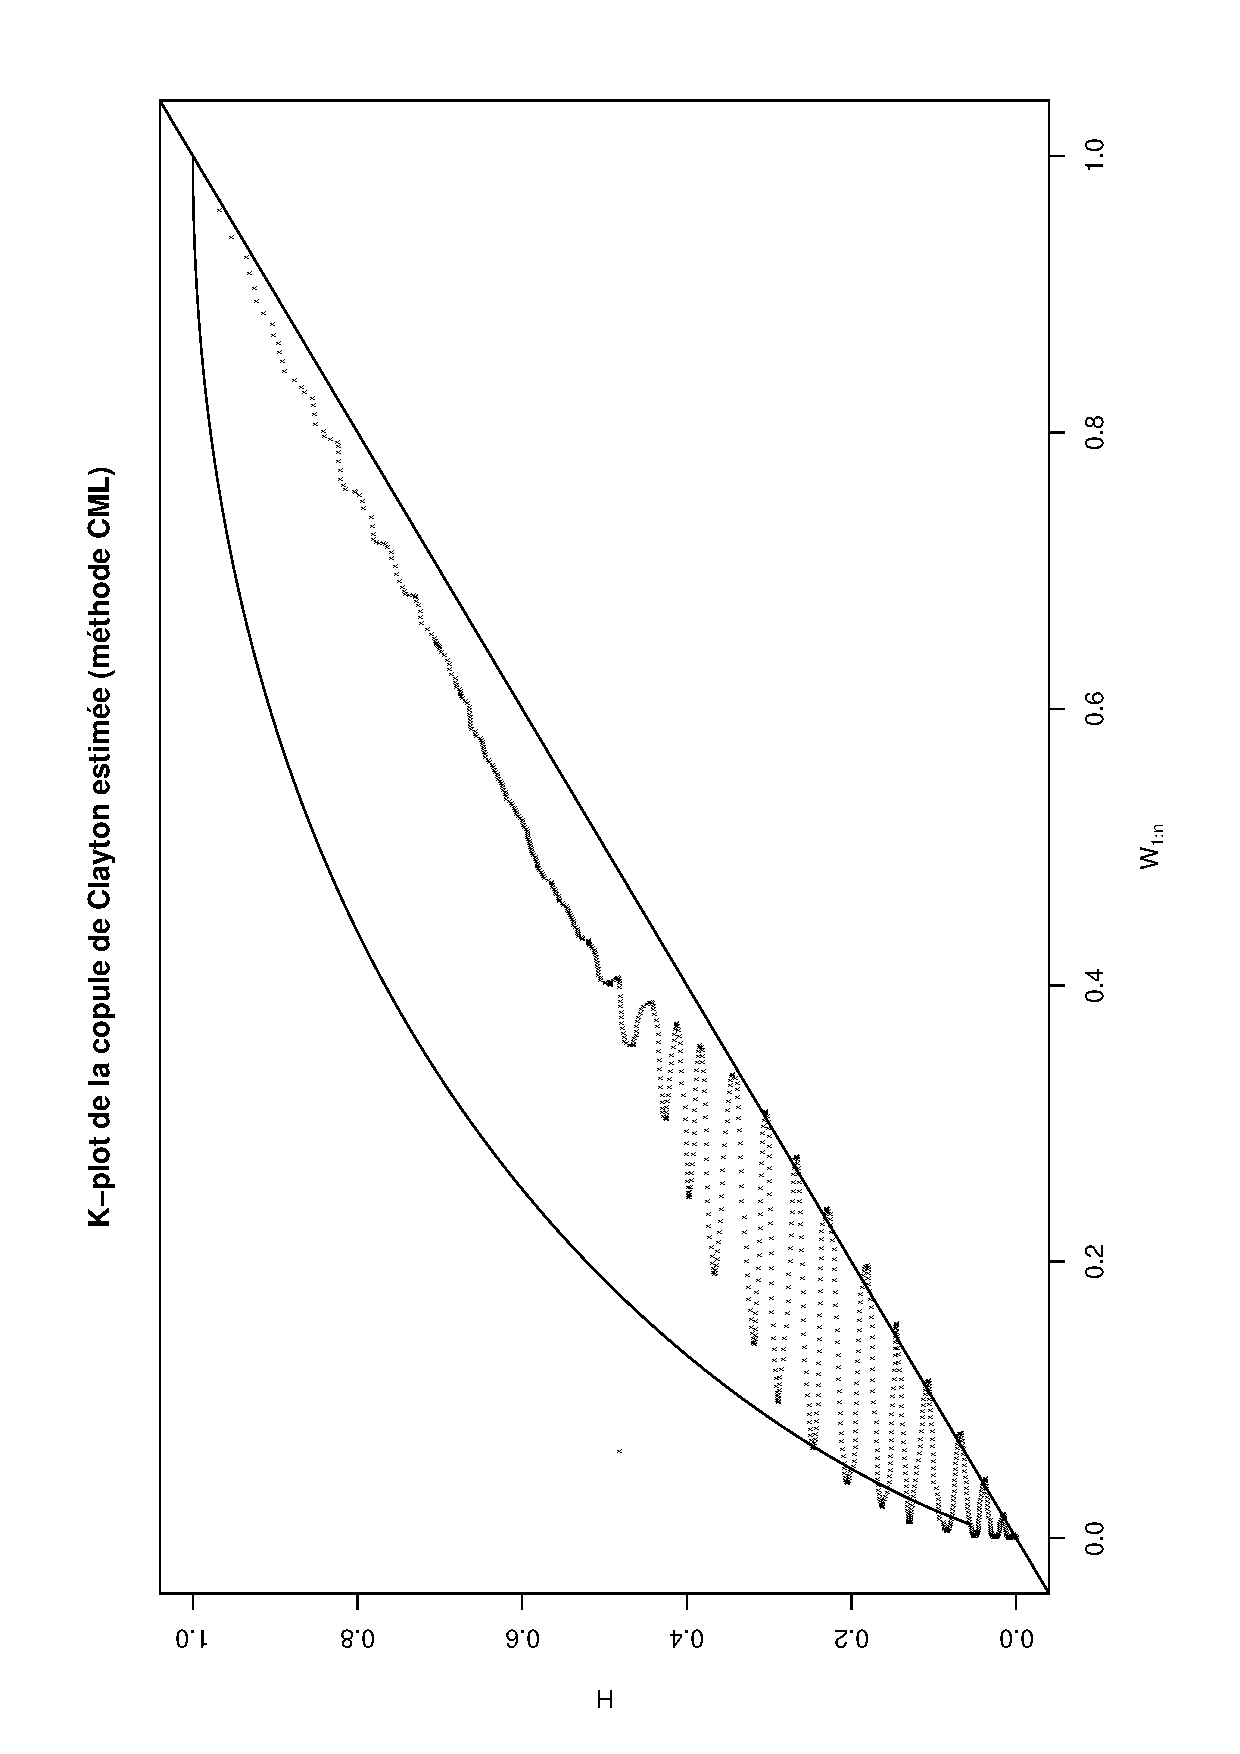
\includegraphics[width=17 cm, angle=0]{./pictures/claytoncmlkplot.png}
      \centering\caption{\label{2}K-plot de la copule de Clayton estimée (méthode CML)}
    \end{center}
\end{figure}

De la même manière, pour ce graphe du K-plot, on observe une similitude et plusieurs disparités par rapport à celui de la copule empirique. En effet, les points semblent se répartir dans le même espace pour les deux figures (globalement entre la courbe de dépendance positive parfaite et la droite d'indépendance $y=x$). Cela montre une nouvelle fois la dépendance positive entre nos deux séries de données. Cependant, concernant le graphe associé à la copule de Clayton estimée, les variations de la répartition des points sont plus grandes et plus nombreuses. Certains points dépassent en effet la courbe de dépendance positive parfaite et on compte également $14$ oscillations distinctes contre $12$ pour le K-plot de la copule empirique. De plus, pour les espérances de la statistique d'ordre des rangs les plus élevés, les points se rapprochent de la droite $y=x$ alors qu'ils sont proches de la courbe de dépendance positive parfaite pour le graphe concernant la copule empirique.

Ces graphes du Khi-plot et K-plot sont donc d'une certaine façon assez éloignés de ceux obtenus pour la copule empirique.

Pour prolonger nos résultats, on réalise également un algorithme de bootstrap paramétrique. Il s'agit de tester l'adéquation à notre modèle de copule. L'hypothèse nulle du test est donc la suivante:
$$
H_0 : C \in (C_{\theta})
$$
Avec $C_{\theta}$ la famille des copules de Clayton dans notre cas. 
En utilisant les mêmes notations que dans le cours, on rejette l'hypothèse nulle si $D_n > L$. 
Dans notre situation, on obtient, avec un seuil de $0,05$, $D_n = 0,1340 > 0,0463 = L$. De plus, la p-value pour cette statistique de Cramer-Von Mises vaut $0$. Avec la fonction \textit{gofCopula} de R, on obtient une p-value de $0,0004$. 
Nous signalons que nous avons codé nous-mêmes l'algorithme du bootstrap paramétrique, la fonction \textit{gofCopula} de R nous permet seulement de vérifier les résultats de notre algorithme.
La copule empirique ne fait donc pas partie de la famille des copules de Clayton.

En conclusion de cette étude sur la copule de Clayton estimée, on peut considérer que la modélisation de la dépendance entre nos deux séries de données par une copule de Clayton n'est pas satisfaisante.

\subsection{Copule de Gumbel}

On procède de la même manière que pour la copule de Clayton. On obtient en sortie de l'algorithme une valeur de $\widehat{\theta}_{CML}=1,4699$ comme estimation du paramètre de la copule de Gumbel par la méthode CML. On a également la valeur de l'écart type $sd = 0,0561$. L'estimation obtenue est ainsi significative. Le maximum de vraisemblance vaut $94,3$.

On représente ainsi ci-dessous les graphes du Khi-plot et du K-plot de la copule de Gumbel estimée:

\noindent%
\begin{figure}[H]
    \begin{center}
      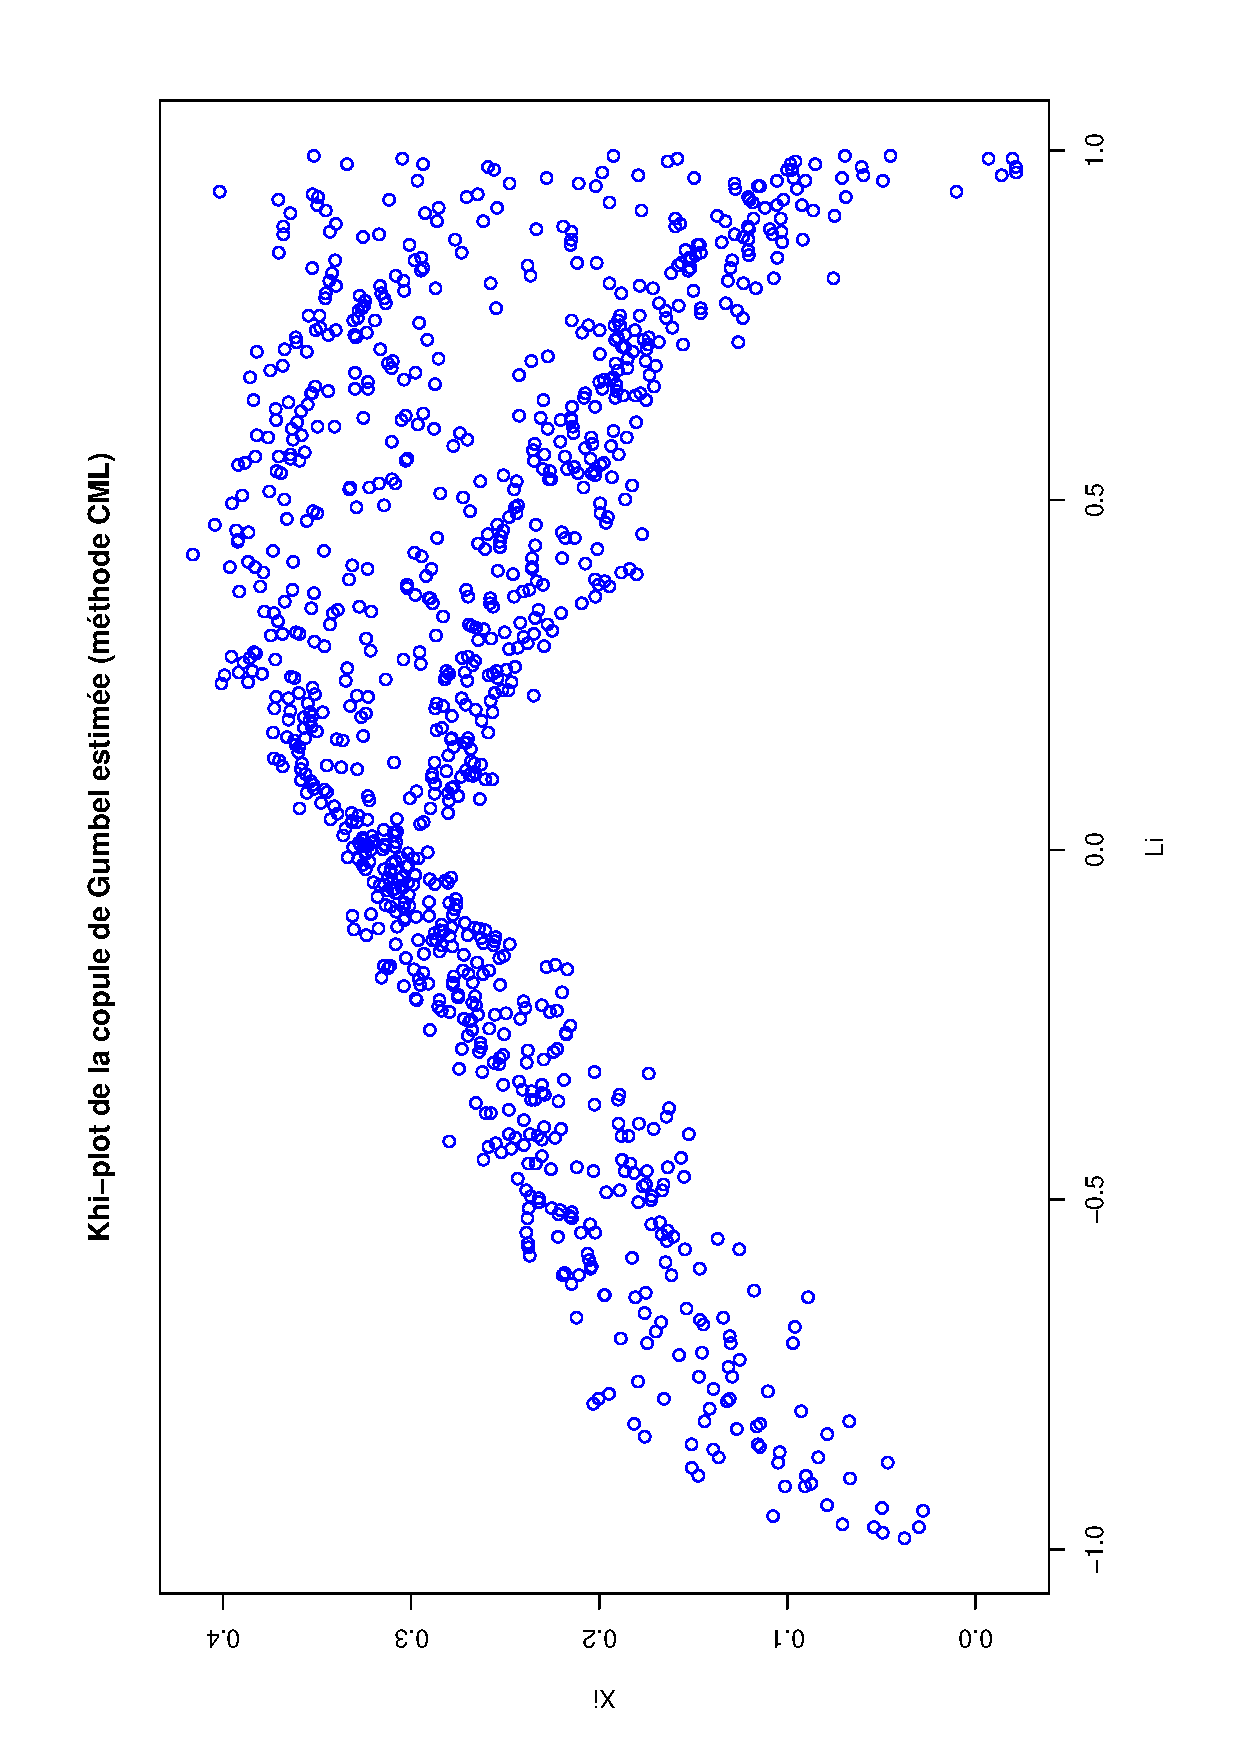
\includegraphics[width=17 cm, angle=0]{./pictures/gumbelcmlkhiplot.png}
      \centering\caption{\label{2}Khi-plot de la copule de Gumbel estimée (méthode CML)}
    \end{center}
\end{figure}

Le Khi-plot ci-dessus est très proche du Khi-plot obtenu avec la copule empirique. En effet, nous avons une répartition des points semblables. Le nuage de points est incurvée de la même manière du coté des valeurs positives des ordonnées et atteint une valeur maximale autour de $0,3$ comme pour le Khi-plot empirique. Certes, nous avons toujours une sorte de séparation en deux du nuage de points pour les valeurs positives en abscisse. Mais, cela est beaucoup moins prononcé que pour le Khi-plot de la copule de Clayton précédent.

\noindent%
\begin{figure}[H]
    \begin{center}
      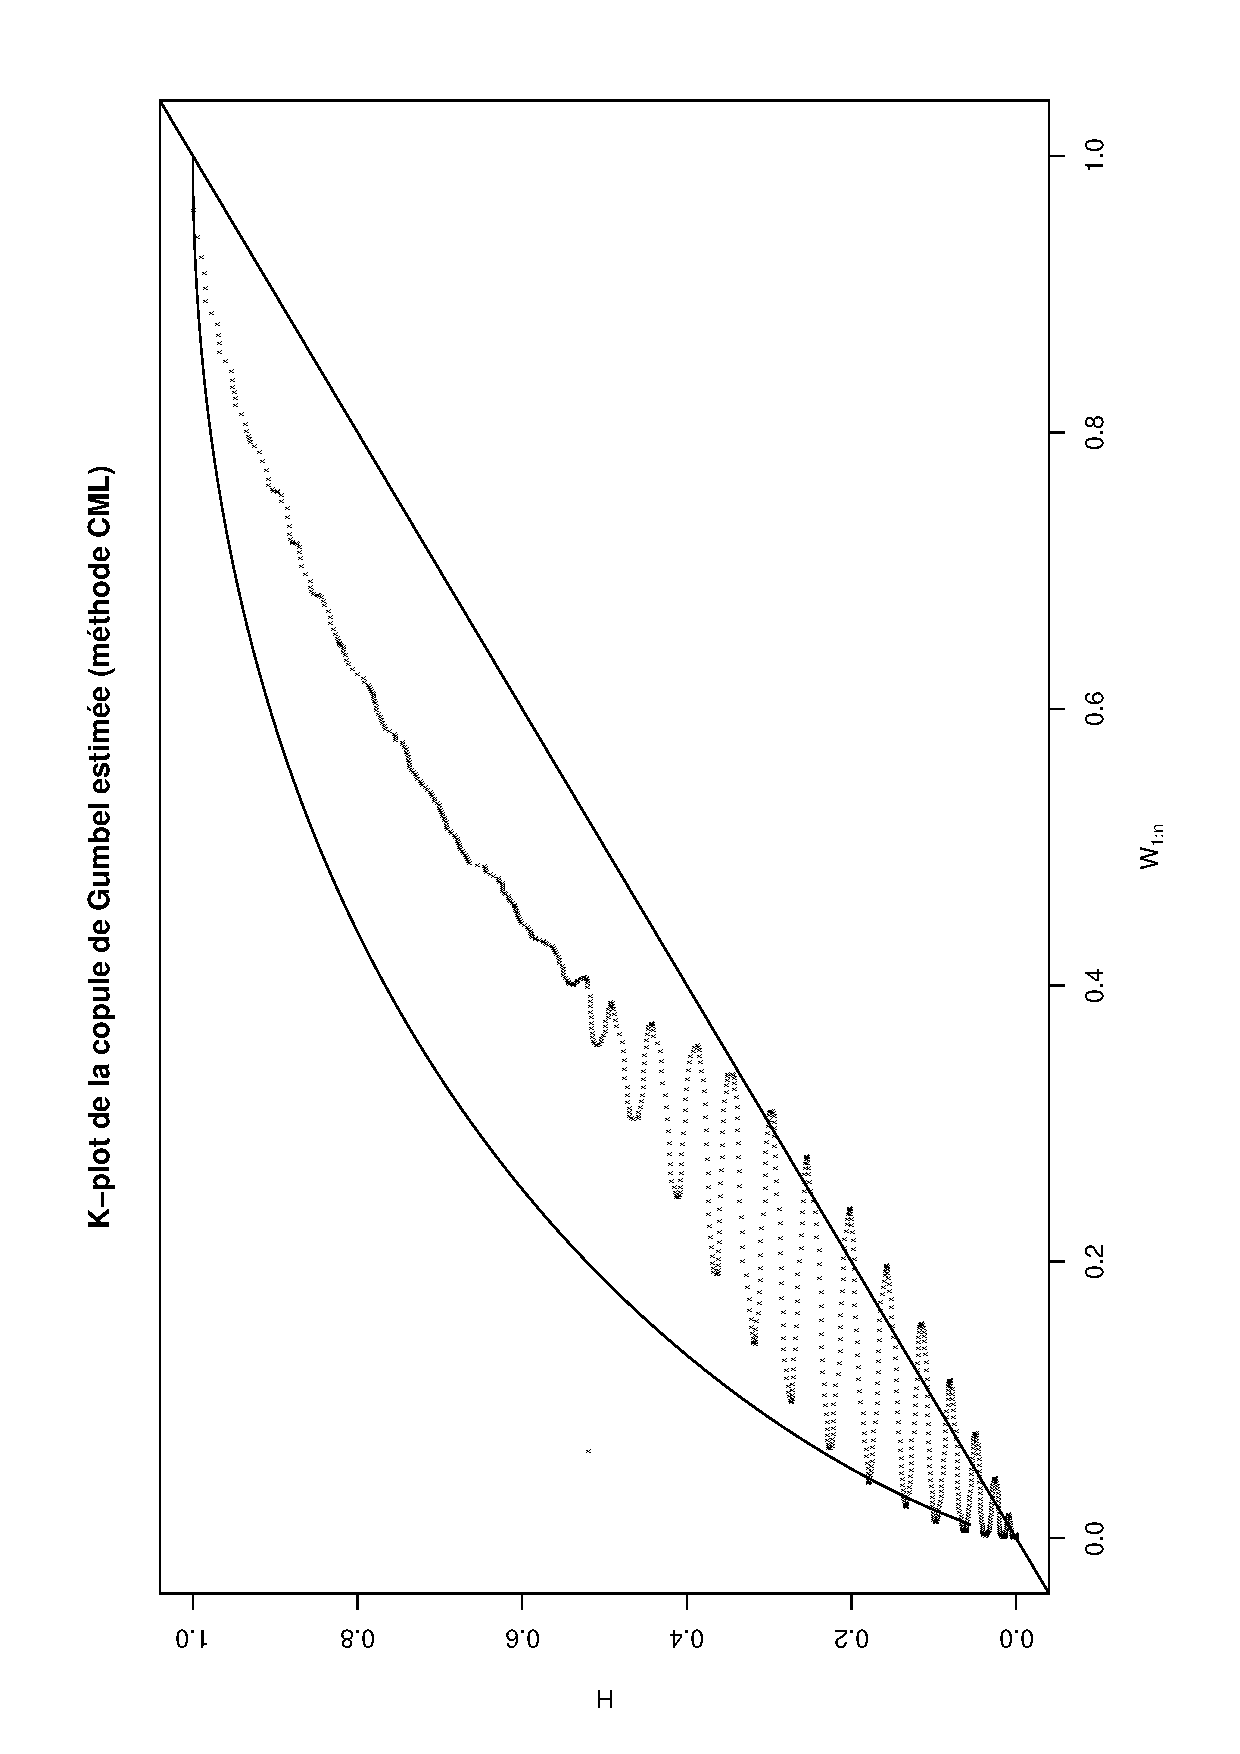
\includegraphics[width=17 cm, angle=0]{./pictures/gumbelcmlkplot.png}
      \centering\caption{\label{2}K-plot de la copule de Gumbel estimée (méthode CML)}
    \end{center}
\end{figure}

Le K-plot de la copule de Gumbel estimée et celui de la copule empirique sont très proches. Les points se répartissent dans le même endroit du graphe (entre la droite $y=x$ et la courbe de dépendance positive parfaite). De plus, on compte le même nombre d'oscillations distinctes ($12$) et les espérances de la statistique d'ordre des rangs les plus élevés sont très proches de la courbe de dépendance positive parfaite pour les deux graphes. 

Les deux graphes précédents semblent donc concordants avec les graphes de la copule empirique.
Cependant, en appliquant l'algorithme du bootstrap paramétrique, on obtient, pour un seuil de 0,05, $D_n = 0,0412 > 0,0325 = L$. On obtient une p-value de $0,01$. Avec la fonction \textit{gofCopula} de R, on obtient une p-value de $0,01249$. 
Nous signalons que nous avons codé nous-mêmes l'algorithme du bootstrap paramétrique, la fonction \textit{gofCopula} de R nous permet seulement de vérifier les résultats de notre algorithme.
Ainsi, on rejette l'hypothèse nulle et on ne peut pas conclure que notre copule empirique fasse partie de la famille des copules de Gumbel.

Ce dernier résultat sur la copule de Gumbel estimée n'est donc pas satisfaisant, alors même qu'il s'agit de la famille de copules qui a été choisie dans le papier de Dutang et Charpentier. Ainsi, nous pouvons voir si d'autres copules peuvent encore mieux s'approcher de la copule empirique.

\subsection{Copule de Frank}

L'estimation du paramètre de la copule de Frank par méthode CML est $\widehat{\theta}_{CML}=3,1729$. L'écart type obtenu est plus élevé que pour les deux études précédentes mais l'estimation reste largement significative. On a $sd = 0,2781$. Le maximum de vraisemblance est égal à $76,04$. Avec cette estimation, nous pouvons simuler des données issues d'une copule de Frank ayant cette valeur de paramètre. On obtient alors les graphes du Khi-plot et K-plot de la copule de Frank estimée ci-dessous:

\noindent%
\begin{figure}[H]
    \begin{center}
      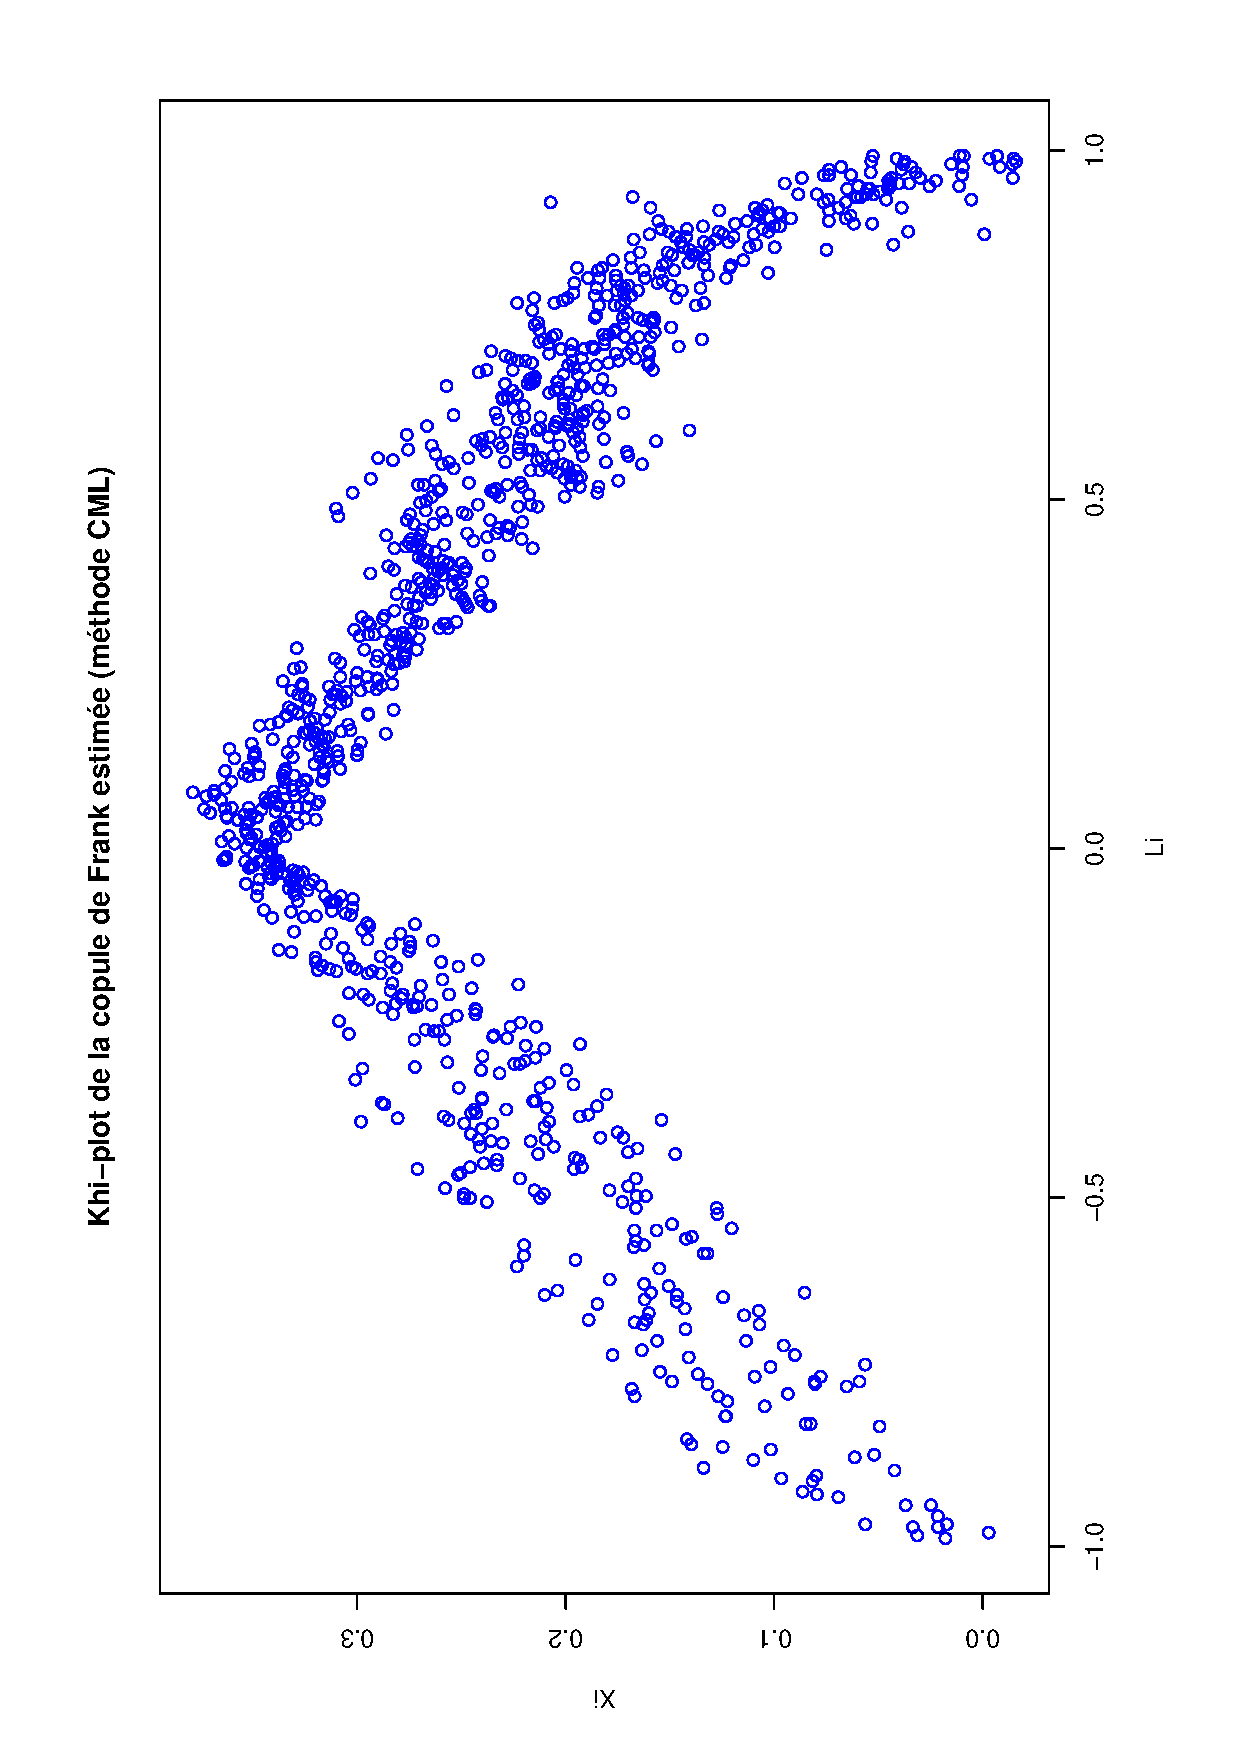
\includegraphics[width=17 cm, angle=0]{./pictures/frankcmlkhiplot.png}
      \centering\caption{\label{2}Khi-plot de la copule de Frank estimée (méthode CML)}
    \end{center}
\end{figure}

Bien que la forme du graphe ci-dessus soit proche de celui effectué pour la copule empirique, on peut remarquer plusieurs différences importantes. Tout d'abord, le Khi-plot de la copule de Frank estimée est beaucoup trop "pentu" par rapport à celui de la copule empirique. Les valeurs aux extrêmes ont une ordonnée autour de $0$ et le maximum en ordonnée dépasse les $0,3$ alors que, pour le graphe de la copule empirique, la valeur maximale en ordonnée est autour de $0,3$ et les valeurs aux extrêmes en abscisse sont autour de $0,1$.

\noindent%
\begin{figure}[H]
    \begin{center}
      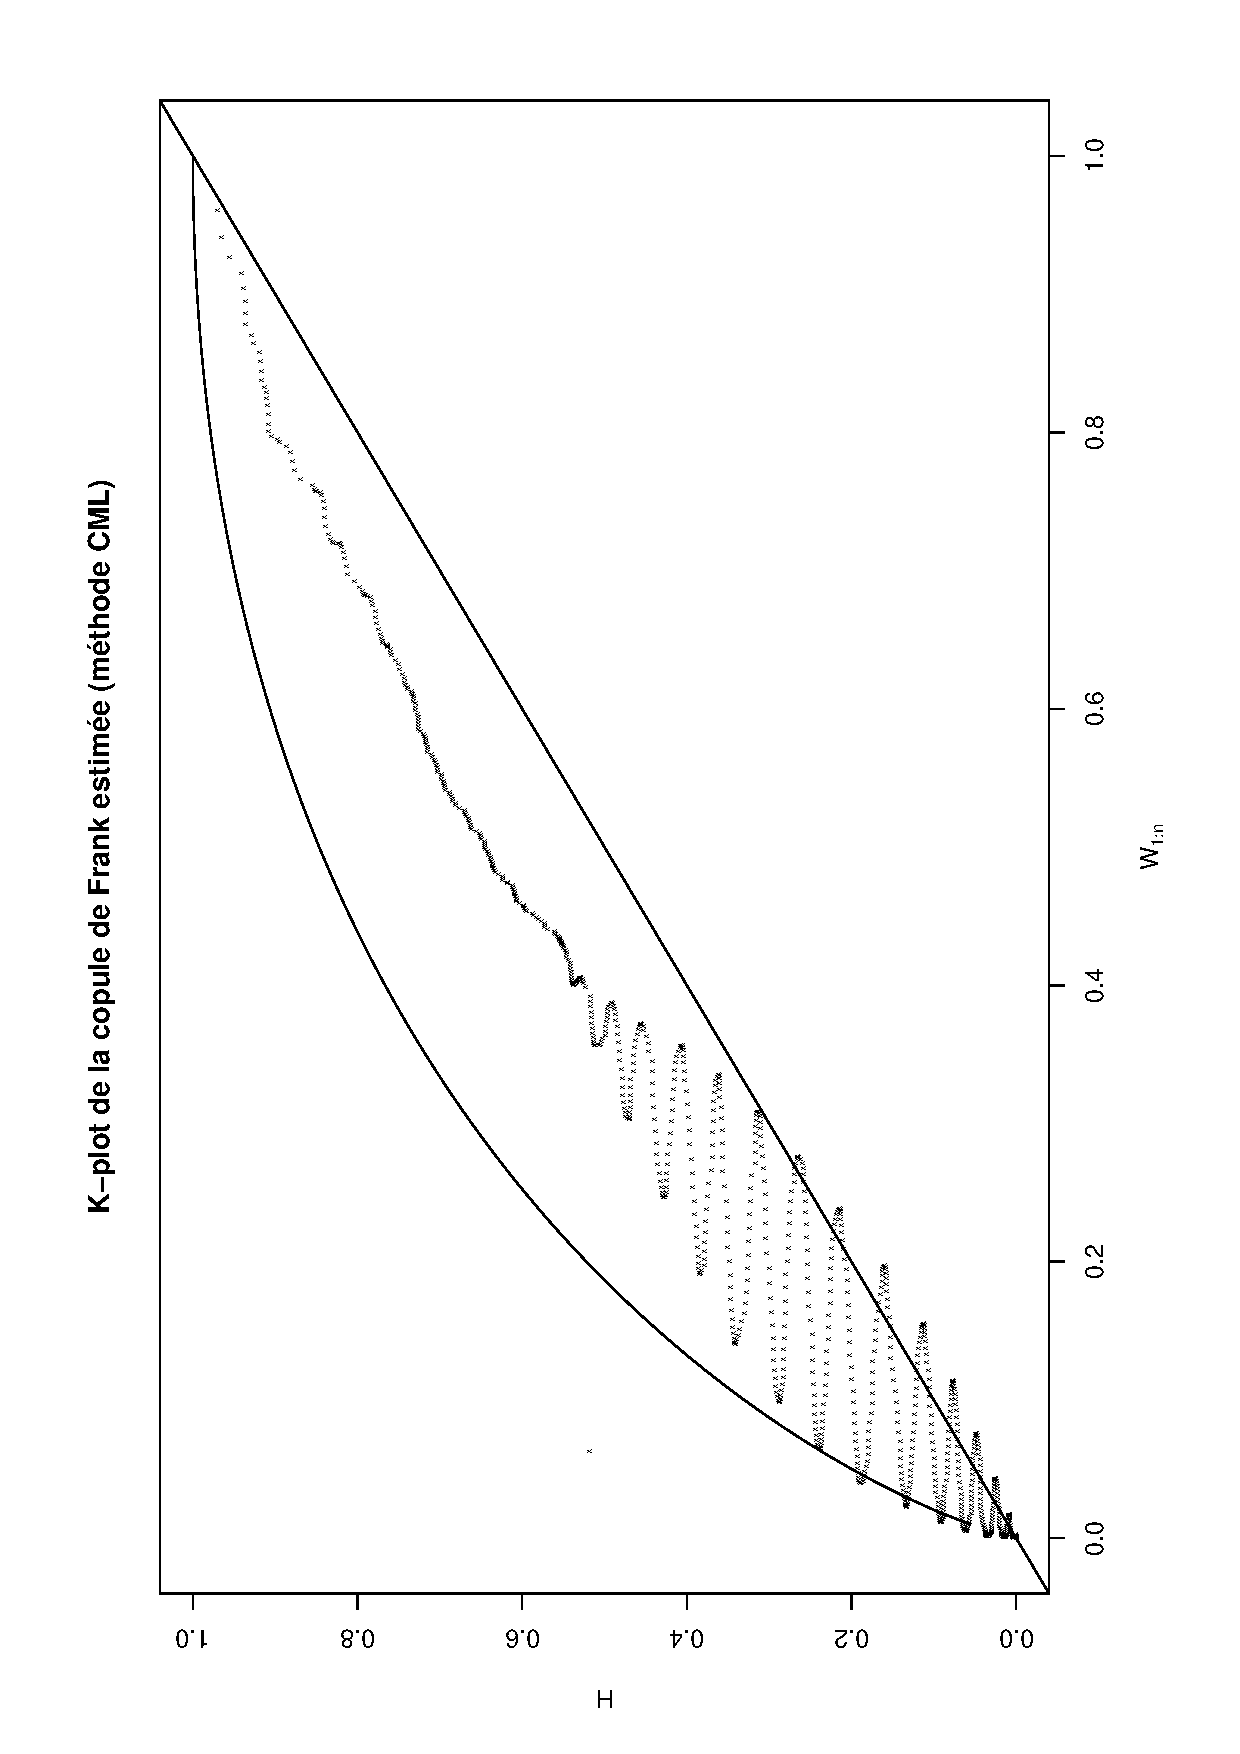
\includegraphics[width=17 cm, angle=0]{./pictures/frankcmlkplot.png}
      \centering\caption{\label{2}K-plot de la copule de Frank estimée (méthode CML)}
    \end{center}
\end{figure}

Le K-plot de la copule de Frank est assez similaire à celui de la copule de Clayton et présente donc les mêmes disparités par rapport à celui de la copule empirique. La différence la plus importante est que, pour les espérances de la statistique d'ordre des rangs les plus élevés, les points se rapprochent de la droite $y=x$ alors qu'ils sont proches de la courbe de dépendance positive parfaite pour le graphe concernant la copule empirique.

Ces graphes du Khi-plot et K-plot sont donc assez éloignés de ceux obtenus pour la copule empirique.

Cela est confirmé par l'algorithme du bootstrap paramétrique. On obtient $D_n = 0,050 > 0,025 = L$, pour un seuil de $0,05$. La p-value est nulle. Avec la fonction \textit{gofCopula} de R, on obtient une p-value de $0,0045$. 
Nous signalons que nous avons codé nous-mêmes l'algorithme du bootstrap paramétrique, la fonction \textit{gofCopula} de R nous permet seulement de vérifier les résultats de notre algorithme. 
Ainsi, on rejette l'hypothèse nulle et on conclut que la copule empirique ne fait pas partie de la famille des copules de Frank.

\subsection{Copule normale}

Par la méthode CML, on obtient l'estimation suivante du paramètre de la copule normale: $\widehat{\theta}_{CML}=0,51412$. L'écrat type associé vaut $sd = 0,031$, ce qui prouve la significativité de l'estimation obtenue. On obtient $94,83$ comme maximum de vraisemblance. 

Comme dans les études précédentes, on trace le Khi-plot et K-plot de la copule normale estimée et on les compare à ceux de la copule empirique.

\noindent%
\begin{figure}[H]
    \begin{center}
      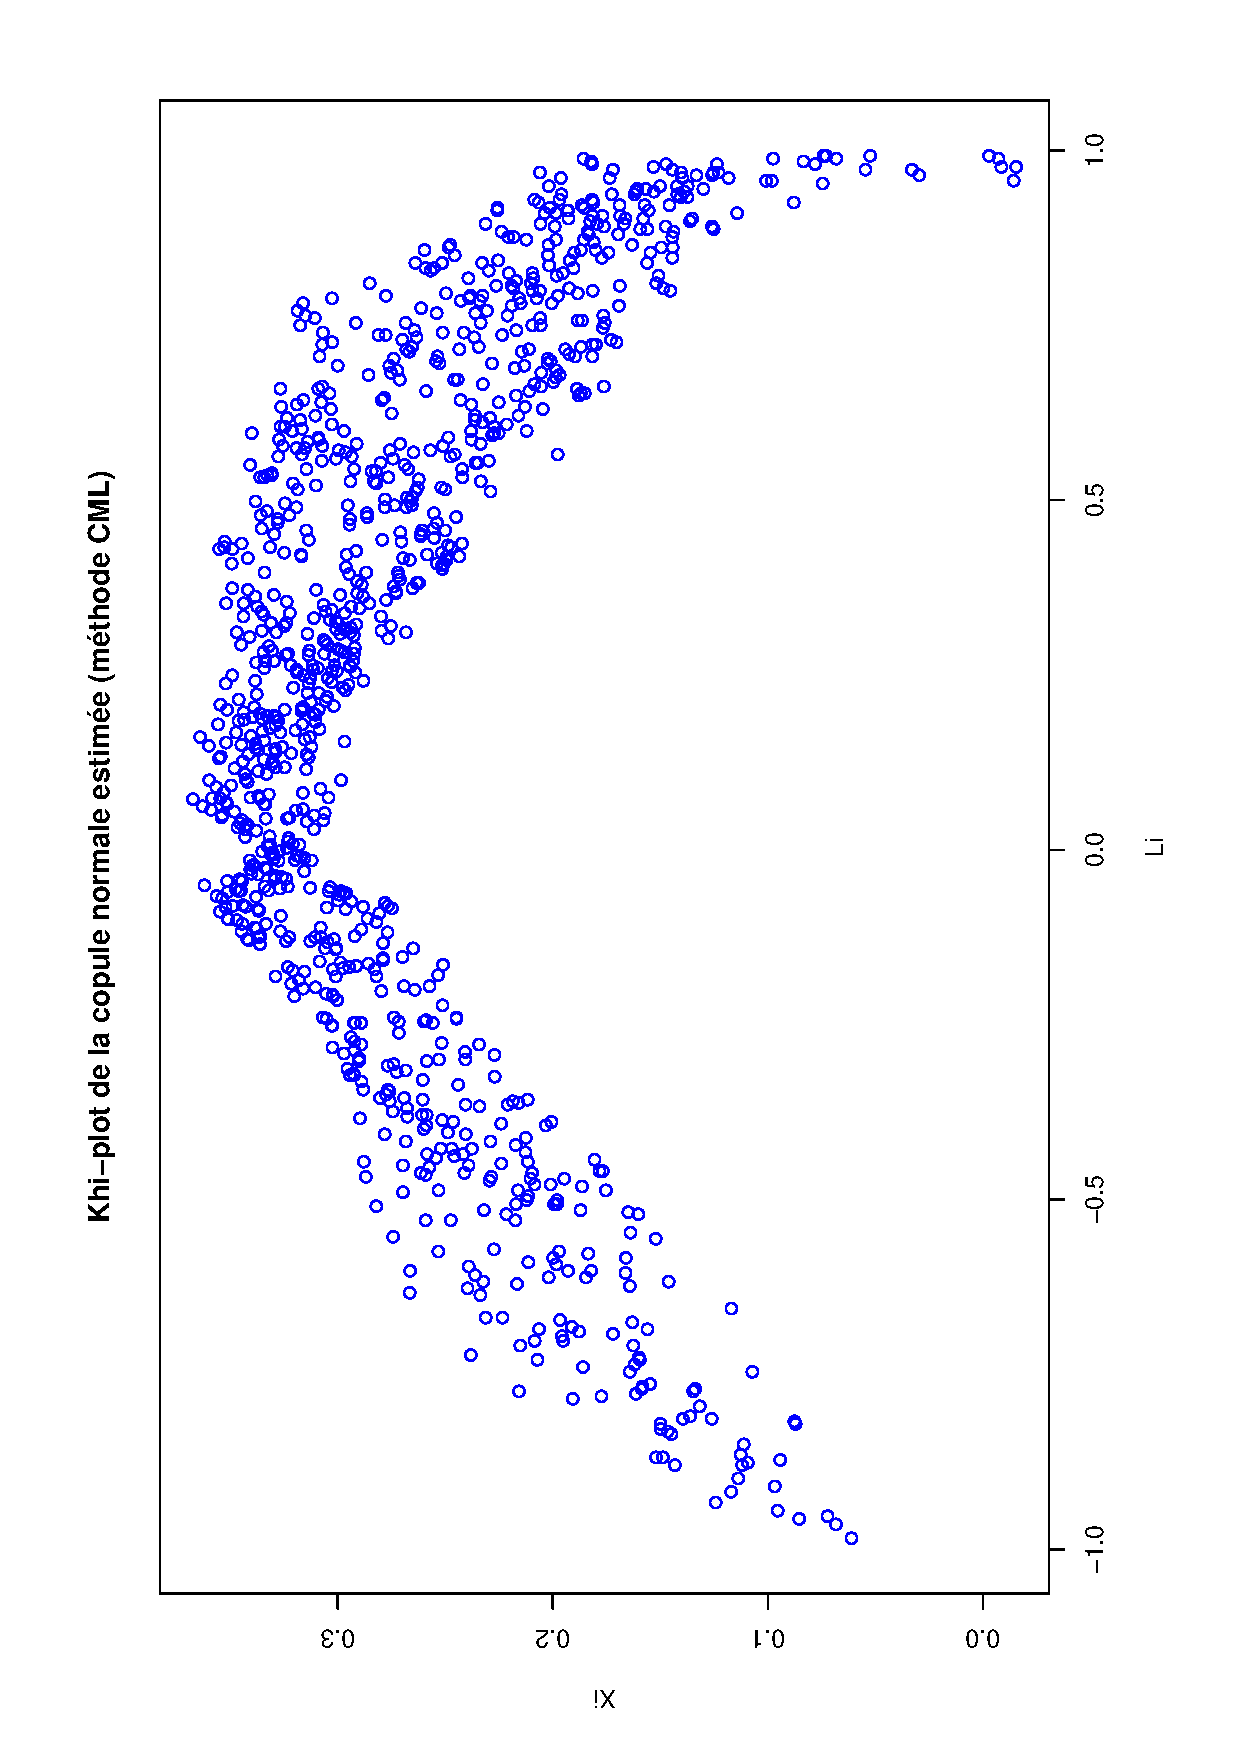
\includegraphics[width=17 cm, angle=0]{./pictures/normalcmlkhiplot.png}
      \centering\caption{\label{2}Khi-plot de la copule normale estimée (méthode CML)}
    \end{center}
\end{figure}

Le Khi-plot de la copule normale estimée est très proche de celui de la copule empirique. On retrouve, sur les deux graphes, la même forme globale du nuage de points. De plus, pour les deux, le maximum en ordonnée est autour de $0,3$ et les valeurs extrêmes des abscisses ont une ordonnée autour de $0,1$. 

\noindent%
\begin{figure}[H]
    \begin{center}
      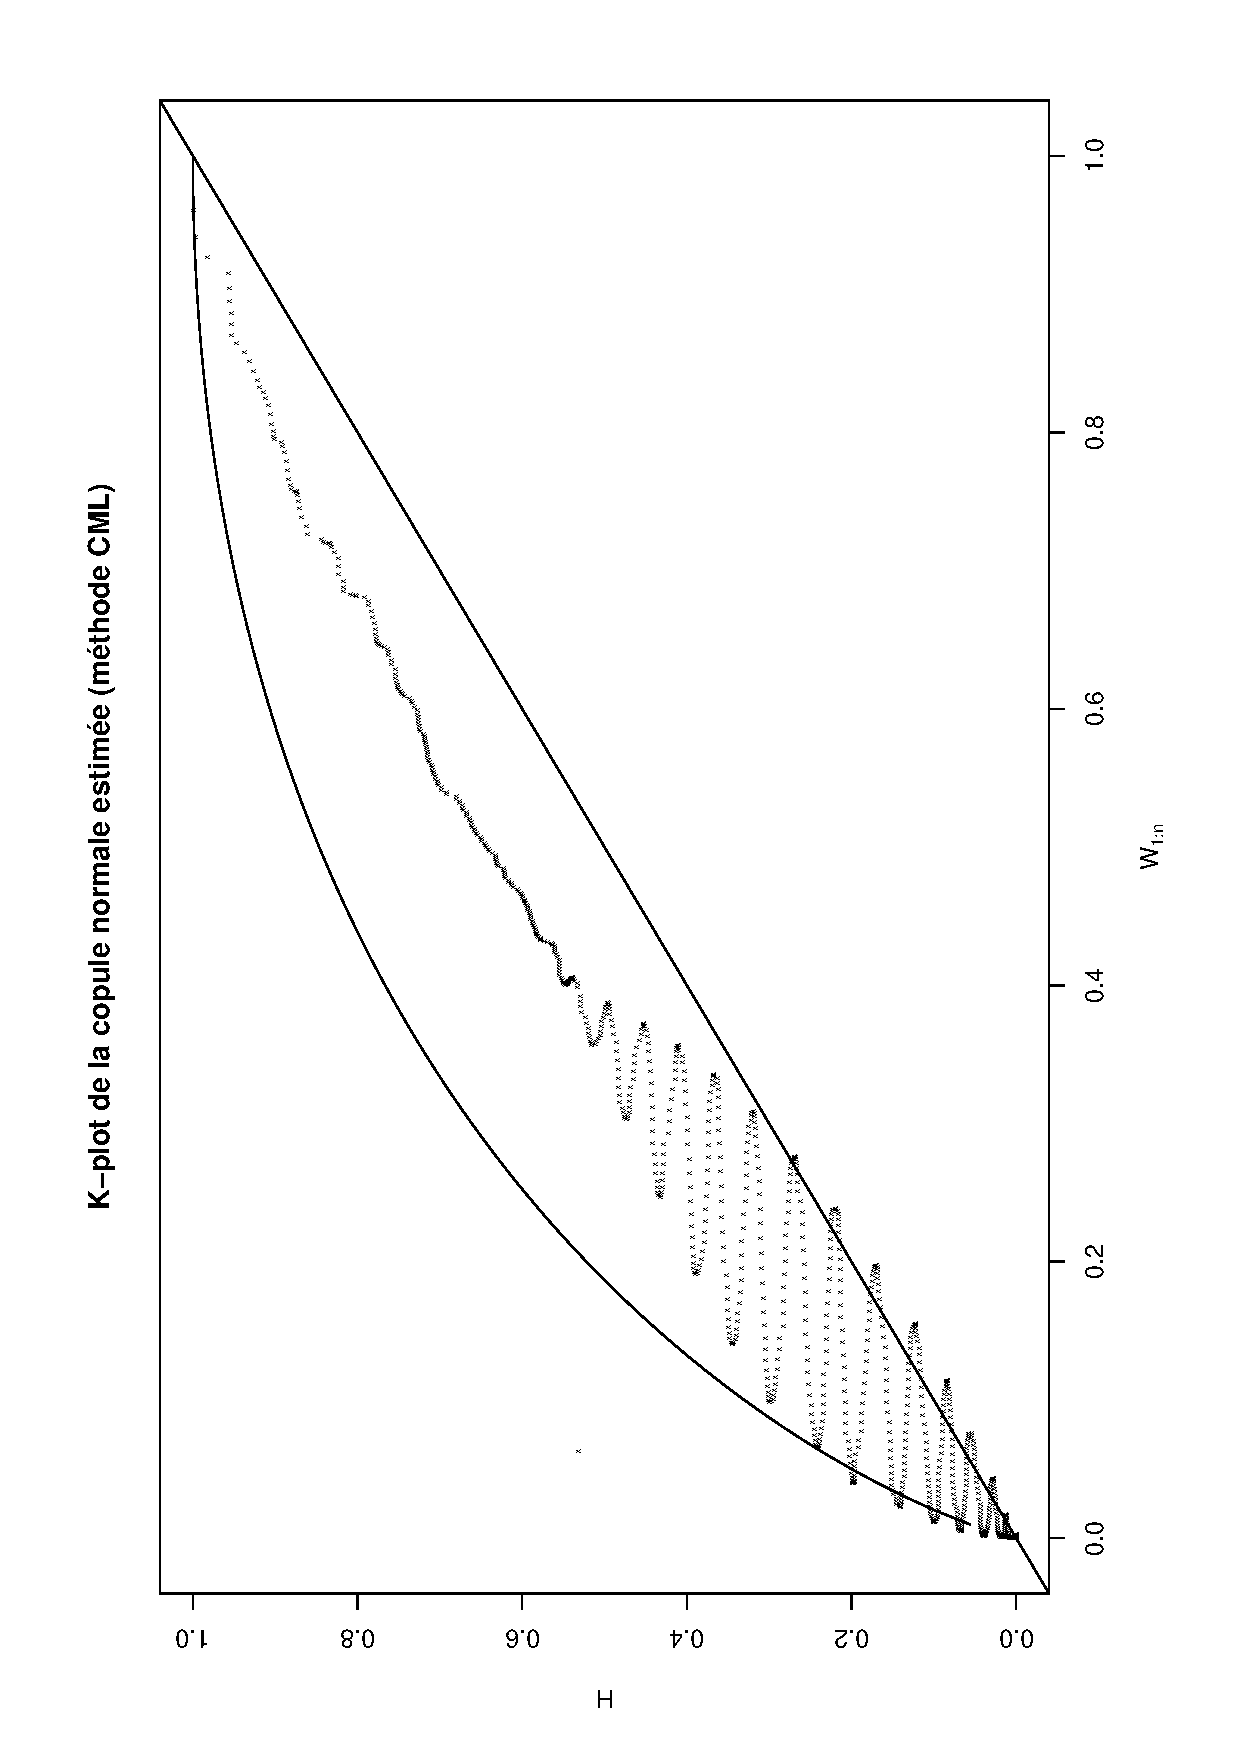
\includegraphics[width=17 cm, angle=0]{./pictures/normalcmlkplot.png}
      \centering\caption{\label{2}K-plot de la copule normale estimée (méthode CML)}
    \end{center}
\end{figure}

Concernant le K-plot de la copule normale estimée, il présente quelques différences avec celui associée à la copule empirique. En effet, les oscillations que l'on observe sont beaucoup plus fortes sur le K-plot de la copule normale estimée. De plus, pour ce K-plot, les espérances de la statistique d'ordre des rangs les plus élevés s'approchent de la courbe de dépendance positive maximale mais de façon plus atténuées que pour le K-plot de la copule empirique.

En résumé, bien que le Khi-plot de la copule normale soit très ressemblant avec celui de la copule empirique, le K-plot, lui, ne nous permet pas de conclure. L'algorithme du bootstrap paramétrique va ainsi nous permettre d'affirmer ou non si la copule empirique fait partie de la famille des copules normales. En sortie de cet algorithme, on a, pour un seuil de $0,05$, $D_n = 0,0314 < 0,0320 = L$. De plus, on obtient une p-value de $0,06$. Avec la fonction \textit{gofCopula} de R, on obtient une p-value de $0,05544$. 
Nous signalons que nous avons codé nous-mêmes l'algorithme du bootstrap paramétrique, la fonction \textit{gofCopula} de R nous permet seulement de vérifier les résultats de notre algorithme. 
On accepte ainsi l'hypothèse nulle et la copule empirique appartient bien à la famille des copules normales.

\subsection{Copule de Student}



\section{Méthode des moments : inversion du tau de Kendall}
%%%%%%%%%%%%%%%%%%%%%%%%%%%%%%%%%%%%%%%%%%%%%%%%%%%%%%%%%%%%%%%%%%%%%%%

Dans cette partie, nous utiliserons la méthode des moments pour estimer le paramètre des copules retenues afin de modéliser la dépendance entre les données sur Saint-Martin et celles sur Echirolles.

\subsection{Copule de Clayton}

\subsection{Copule de Gumbel}

\subsection{Copule de Frank}

\subsection{Copule normale}

\subsection{Copule de Student}

\section{Test graphique d'adéquation à la copule : le Kendall plot}
%%%%%%%%%%%%%%%%%%%%%%%%%%%%%%%%%%%%%%%%%%%%%%%%%%%%%%%%%%%%%%%%%%%%%%%

\subsection{Dépendogramme empirique et dépendogramme théorique}

\subsection{K-plot}

\section{Test statistique d'adéquation à la copule : le Kendall plot}
%%%%%%%%%%%%%%%%%%%%%%%%%%%%%%%%%%%%%%%%%%%%%%%%%%%%%%%%%%%%%%%%%%%%%%%

\subsection{Test de Kolmogorov-Smirnov}

\subsection{La statistique de Cramér-von Mises}

\subsection{Estimation du seuil critique par bootstrap paramétrique}





TODO   TODO   TODO   TODO



%% \noindent%
%% \begin{figure}[H]
%%     \begin{center}
%%       \includegraphics[width=17 cm, angle=0]{./pictures/logchrono1.png}
%%       \centering\caption{\label{2}Logarithme du total des importations de gaz naturel}
%%     \end{center}
%% \end{figure}

  \cleardoublepage
  %\include{latex_files/partie2}
  % \cleardoublepage
  %\include{latex_files/partie3}
  % \cleardoublepage
  %\include{latex_files/partie4}
   %\cleardoublepage
  \section*{Conclusion}
\addcontentsline{toc}{section}{Conclusion}

Lors de ce projet, nous avons pu mettre en application la théorie des copules. Cette théorie voit tout son intérêt dans la gestion des risques et plus généralement dans le domaine de l'actuariat et de la finance. Grâce à ce puissant outil statistique, nous avons cherché à proposer une modélisation de la dépendance entre les valeurs de la vitesse maximale du vent enregistrées par deux stations distinctes. Les procédures d'estimation des copules ont été réalisées selon diverses méthodes (paramétriques, semi-paramétriques et non-paramétriques) afin d'estimer au mieux les paramètres de chaque copule (et les paramètres des lois marginales). Ensuite, nous avons retenu la moyenne des paramètres obtenu par ces différentes méthodes pour réaliser un ensemble de tests graphiques et de tests statistiques afin de comparer l'adéquation des modèles de copules étudiés à nos données. Ainsi, il ressort de cette étude que la copule normale permet de représenter au mieux la dépendance positive existant entre les valeurs des deux stations.





\clearpage

\clearpage
%% ANNEXE
\appendix
%\section{Annexe}
%\label{refCode}
\begin{lstlisting}[language=cli, name=Sim, caption=Code R]


\end{lstlisting}


\cleardoublepage
   \phantomsection\addcontentsline{toc}{section}{Références}
\begin{thebibliography}{ABC}	
%%    \bibitem[REF]{reference} auteur. \emph{titre}. édition, année.
%%    \bibitem[LPP]{lpp} Rolland. \emph{LaTeX par la
%%    pratique}. O'Reilly, 1999.


\bibitem{reference}\label{ref1} E. Masiello, \emph{Inférence statistique des copules}, ISFA, support de cours, 2014-2015.

\bibitem{reference}\label{ref2} A. Charpentier, C. Dutang, \emph{L'actuariat avec R}, version numérique, décembre 2012.

\bibitem{reference}\label{ref3} T. Roncalli, \emph{Gestion des risques multiples ou copules et aspects mutidimensionnels du risque}, ENSAI, support de cours, 2002.

\bibitem{reference}\label{ref4} M-C. Brassier, G. Depommier, P. Sloma, \emph{Copules et dépendance entre les risques}, ALTIA, séminaire, 2010.

\bibitem{reference}\label{ref1} F. Planchet, \emph{Dépendance stochastique, introduction à la théorie des copules}, ISFA, support de cours, 2010-2011.

\end{thebibliography}

%% \textbf{Sources des données financières sur l'inflation} :

%% \url{www.inflation.eu}


%% \include{latex_files/partie5}
%%    \cleardoublepage
%%%%%%%%%%%%%%%%% FIN DU DOCUMENT %%%%%%%%%%%%%%%%%%%%%%

\end{document}


